%% josis.tex 1.4   2016-09-15    JoSIS latex template
%------------------------------------------------------------------
% Filename: josis_template.tex
%
% This file is intended as a template for typesetting articles for the
%
%                        Journal of Spatial Information Science.
%
% Please edit this template to generate your own formatted manuscripts
% for submission to JOSIS. See http://josis.org for further details.
%


%%% JOSIS checks in typesetting
%%% * All titles and sections lower case *EXCEPT short title  [ ]
%%% * Remove author postal addresses, only have geographic places and institutions [ ] 
%%% * Consistent use of Section, Figure, Table (capitalized and in full) [ ]
%%% * 10 keywords (and all lower case) [ ]
%%% * Remove all avoidable footnotes [ ]
%%% * Use double quotation marks (``'' not "" or `') [ ]
%%% * Punctuation inside quotations [ ]
%%% * E.g. and i.e. followed by comma [ ]
%%% * cf. followed by tilde [ ]
%%% * Itemize and enumerate correctly punctuated [e.g., "1. x, 2. y, and 3. x." ]
%%% * And/or lists using American English punctuation (e.g., "x, y, and z") [ ] 
%%% * Bibliography (e.g., en-dashes for number ranges, consistent "Proc.~" for Proceedings of..., etc.) []
%%% * Acknowledgment style use section* [ ] 
%%% * et al. no italics, but with dot  [ ] 
%%% * All captions end with full stop  [ ] 
%%% * Table captions under, not over table  [ ]
%%% * Adjust urls with burlalt [ ] 
%%% * Check correct use of hyphens, emdashes, endashes  [ ]
%%% * Perform spell check  [ ] 

%%% JOSIS checks directly before publication 
%%% Check DOI, page numbers on article and web site. [ ]
%%% Update web site with final title, abstract, keywords. [ ] 
%%% Build with distiller for DOI links. [ ]


% Required documentclass definition for JOSIS
\documentclass{josis}
\usepackage{hyperref}
\usepackage[hyphenbreaks]{breakurl}
\usepackage{booktabs}
\usepackage{stmaryrd}
\usepackage[T1]{fontenc}
\usepackage{cite}
\usepackage{subcaption}

% Suggested packages for algorithm formatting
\usepackage{algorithm}
%\usepackage{algorithmic}
\usepackage{algpseudocode}
\usepackage{pythonhighlight}

\usepackage{amssymb,amsmath}
%\usepackage[table]{xcolor}
\usepackage{lastpage}
\renewcommand{\topfraction}{0.9} 
\renewcommand{\textfraction}{0.1}
% Page setup and overhangs
\sloppy
\widowpenalty=10000
\clubpenalty=10000
\hyphenpenalty=75

% Article details for accepted manuscripts will be added by editorial staff
% Omit year if article in press
% Omit number if article under review
\josisdetails{%
   number=2, year=2024, firstpage=1, lastpage=\pageref{LastPage}, 
  doi={IUCP-2024},
  % received={December 24, 2015}, 
   %returned={February 25, 2016},
   %revised={July 13, 2016},
   %accepted={September 5, 2016},
   }

%\newcommand{\mydoi}[1]{\href{http://dx.doi.org/#1}{doi:\protect\detokenize{#1}}}

%\renewcommand{\UrlLeft}{http:\sslash}
%\DeclareUrlCommand\myurl{\def\UrlLeft{}\def\UrlRight{}%
%\urlstyle{tt}}

\urlstyle{rm}
\makeatletter
% Inspired by http://anti.teamidiot.de/nei/2009/09/latex_url_slash_spacingkerning/
% but slightly less kern and shorter underscore
\let\UrlSpecialsOld\UrlSpecials
\def\UrlSpecials{\UrlSpecialsOld\do\/{\Url@slash}\do\_{\Url@underscore}}%
\def\Url@slash{\@ifnextchar/{\kern-.11em\mathchar47\kern-.2em}%
    {\kern-.0em\mathchar47\kern-.08em\penalty\UrlBigBreakPenalty}}
\def\Url@underscore{\nfss@text{\leavevmode \kern.06em\vbox{\hrule\@width.3em}}}
\makeatother

\hypersetup{
colorlinks=true,
linkcolor=black,
citecolor=black,
urlcolor=black
} 

% Add the running author and running title information
\runningauthor{\begin{minipage}{.9\textwidth}\centering Ashly Biju, Aiswarya Lakshmi , Jiya Mary Joby \end{minipage}}
\runningtitle{Fake News Detection}

% Document begins
\begin{document}
%\setcounter{page}{33}


% Insert your own title
\title{Fake News Detection Using {\texttt{Python}} and Machine Learning}

% Insert your manuscipts authors, affiliations, and addresses
\author{Ashly Biju}
\author{Jiya Mary Joby }
\author{Aiswarya Lakshmi}\affil{Saintgits Group of Institutions, Kottayam, Kerala}
\date{}
\maketitle
% Add 5-10 keywords for every submission
\keywords{fake news,true news, tokenization, stemming, lemmetaization, vectorization, TFD-IDF, classification, Large Language Models, transformers, BERT}
% Add a short abstract of 150-250 words 
\begin{abstract}
With the advancement of social media and online platforms,the spread of fake news has become a major concern. Fake news simply means `wrong information’ that can have real world adverse effects and can be difficult to distinguish from real news.Therefore, it is a research challenge to validate the source, content, and publisher of a news article before classifying it as genuine or fake. The existing systems and techniques are not efficient enough to accurately classify a given news based on its statistical rating.In this adverse situation, machine learning techniques can be used to detect fake news. Machine learning plays an imperative role in categorizing news data and information, despite some limitations. In this work,we propose a system for fake news detection that uses machine learning techniques implemented in Python. We propose a dataset of fake and true news to train the proposed system. 
\end{abstract}
% Your main text begins here. 
\section{Introduction}
In today‘s society,social media is the most easy and convenient way of sharing news to each other.So most of the news consumption by people is through different social media platforms. The term ‘fake news’ became more relevant after the advancement of social media platforms \cite{baarir2021fake}. This fake news not just adversely affect an individual but it also affects the society as a whole.  The right to information is basic right and it is more important that we get the true information. Thus, it is very important to stop the chain of fake news from the root itself.  This is where our project will be beneficial. This project uses machine learning principles and algorithms to detect fake news, which can be of great use in the identification of correct information. In this paper, it is sought to produce a model that can accurately predict the likelihood that a given article is fake news harnessing the power of machine language and python and thus prevent the dissemination of fake news to an extent. A comprehensive literature survey is conducted to overview the current status of the research in this area. Z Khanam et al have studied this subject comprehensively and successfully predicted the fake with 92\% accuracy \cite{khanam2021fake}. Iftikhar Ahmad et al have published a work on the same title using ensemble methods with an average accuracy of 90.2\% \cite{ahmad2020fake}. Keeping these works as benchmarks, this project aims for higher accuracy using advanced tools and also provides a practical guideline for using machine learning tools for fake news prediction, considering resources and performance measures.
\section{Libraries Used}
In the project for various tasks, following packages are used.
\begin{python}
    NumPy
    Pandas
    Seaborn
    NLTK
    Matplotlib
    BERT
    Scikit-learn
\end{python}
\section{Methodology}
  In this work two types of models are used. For the first part, various classical Machine Learning models are used. Among them the decision tree classifier is found to be better in terms of accuracy and other performance measures. Various stages in the implementation process are:
\begin{description}
    \item[Data Loading:] Loading the data for the Machine Learning task from reliabile sources.
    \item[Pre-processing \& Data cleaning] In this stage the loaded data will be cleaned and make ready for using Machine Learning algorithm. In text analysis, the text should be properly pre-processed.For pre-processing we use the nltk library.

    \item[Feature extraction:] Term Frequency-Inverse Document Frequency (TF-IDF). Through this step calculate a score for each word based on its frequency in the document and its rarity across all documents.
    \item[Dataset Preparation:]Split the dataset into training and testing sets.
    %\item[Classification:] Implementing various Machine Learning Classification models on the document matrix to classify the input text into fake or true news.
    \item[Model Training:] Choose a classification algorithm, such as Naive Bayes, Logistic Regression, or decision tree and train the model using the training set \& the extracted features.
    \item[Model Evaluation:] Test the trained model on the testing set to evaluate its performance.Use the metrics such as accuracy, precision, recall, and F1-score to assess the model's effectiveness.
    \item[Model selection and reporting] In this final stage, based on various performance measures the better model will be selected and report the model performance matrices.
\end{description} 
\section{Implementation}
As the first step in the task, the two files- {\texttt{fake.csv}} and {\texttt{true.csv}} are loaded into  the Intel's {\texttt{DevCloud -OpenAPI}}for the classification task using the url \url{https://onlineacademiccommunity.uvic.ca/isot/wp-content/uploads/sites/7295/2023/03/News-_dataset.zip}. The {\texttt{.csv}} files are turned into a {\texttt{pands}} DataFrame. Both the datasets are properly labelled and is concatenated to a single dataframe. The EDA on subjects and real and fake news status is shown in Figure \ref{fig:mainfig}.
\begin{figure}
    \centering
    
    \begin{subfigure}[b]{0.45\textwidth}
        \centering
        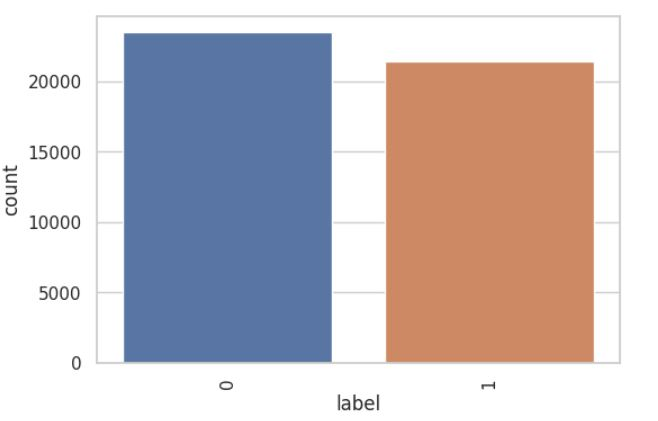
\includegraphics[width=\textwidth]{real_vs_fake.JPG}
        \caption{Real Vs fake news count}
        \label{fig:subfig1}
    \end{subfigure}
    \hfill
    \begin{subfigure}[b]{0.45\textwidth}
        \centering
        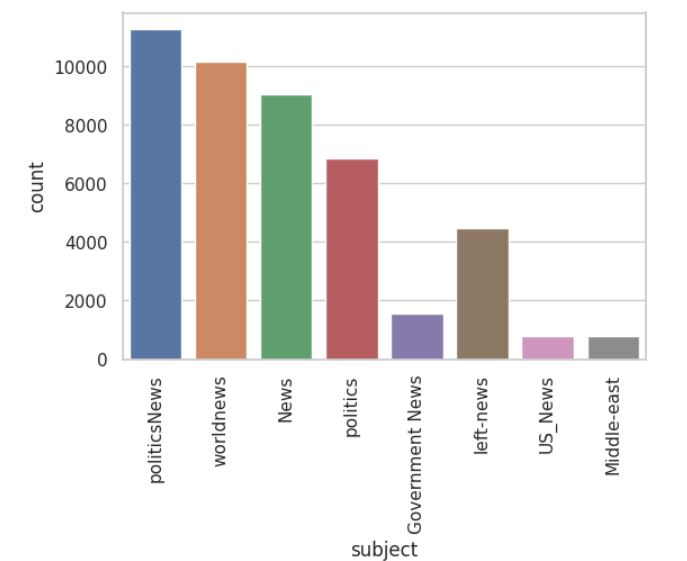
\includegraphics[width=\textwidth]{subject_wise_news}
        \caption{Subject-wise news items in the database}
        \label{fig:subfig2}
    \end{subfigure}
    
    \caption{Type and subject-wise Distribution of news items}
    \label{fig:mainfig}
\end{figure}
From Figure \ref{fig:mainfig}, it is clear that the dataset contains almost equal number of real and fake news feeds and so sufficiently balensed in terms of the class. Further more the most dominating subjects are {\em political news, world news, news and politics}.\\
The pre-processing and cleaning stage is completed in four distinct and consecutive steps:
\begin{itemize}
    \item {\em Tokenization:} Break the text into individual words or tokens.
    \item {\em Lowercasing:} Convert all tokens to lowercase to ensure case insensitivity.
    \item {\em Stopword removal:}Remove common words that do not carry much meaning.
    \item {\em Lemmatization: } Reduce words to their base or dictionary form to normalize the text.
\end{itemize}
The pre-processing stage is completed in $365.365\,sec$ in {\em Google Colaboratoy} and in $243.56\,sec$ in {\em Intel DevCloud}.
The word cloud and word frequency plot of the cleaned data is shown in Figure \ref{fig:mainfig2}.

\begin{figure}
    \centering
    
    \begin{subfigure}[b]{0.45\textwidth}
        \centering
        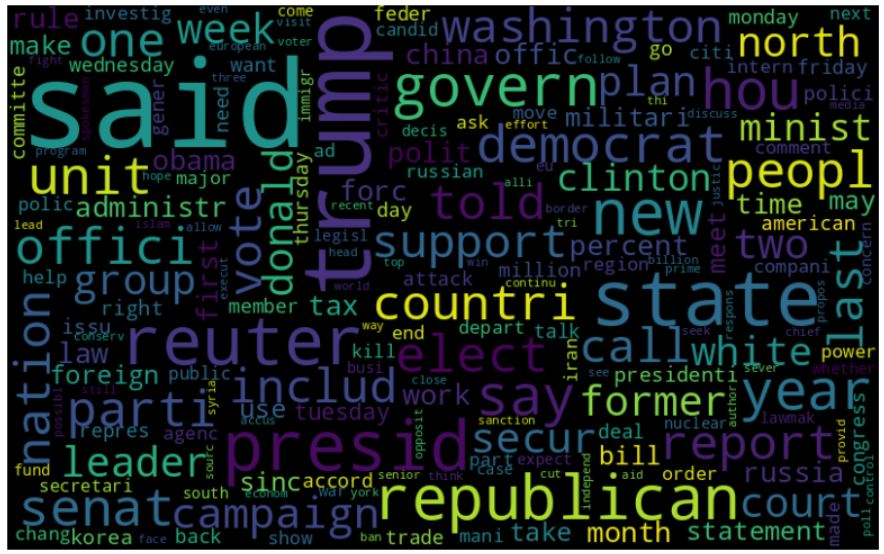
\includegraphics[width=\textwidth]{word_count_after_cleaning.JPG}
        \caption{Word cloud showing cleaned news data}
        \label{fig:subfig3}
    \end{subfigure}
    \hfill
    \begin{subfigure}[b]{0.45\textwidth}
        \centering
        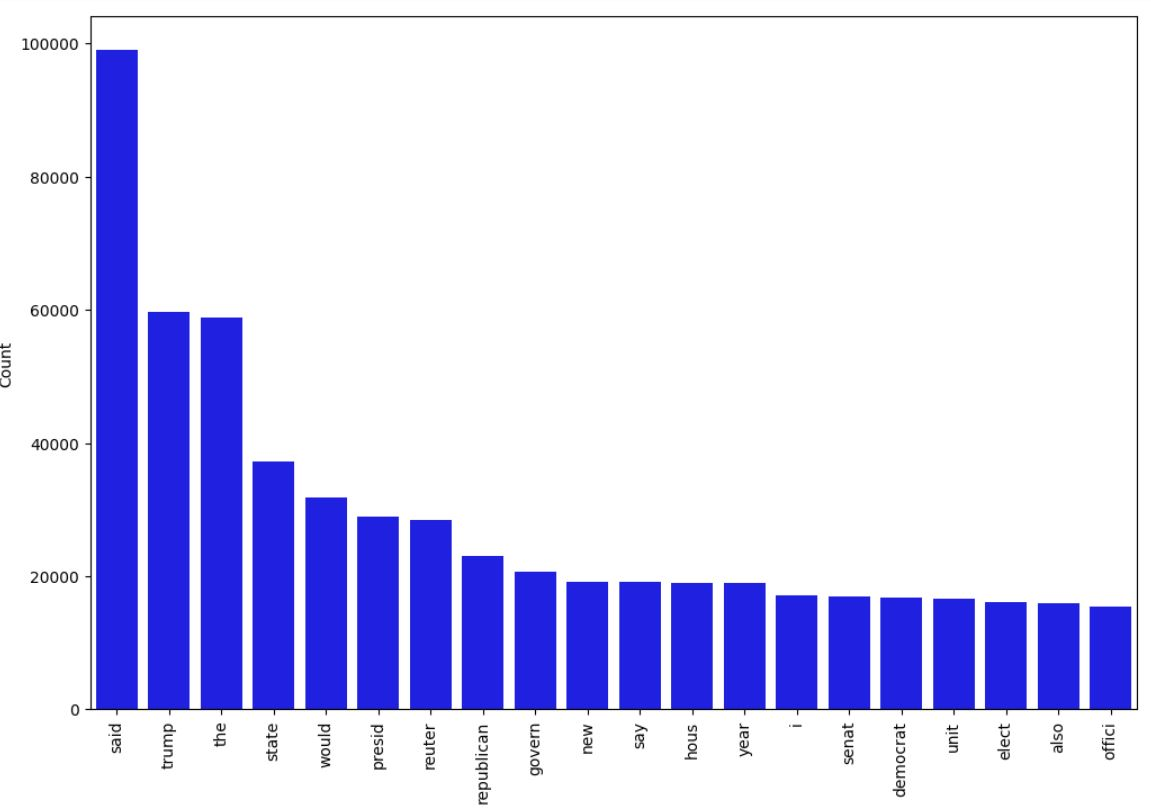
\includegraphics[width=\textwidth]{word_count_after_cleaning1.jpg}
        \caption{Word count plot for cleaned data}
        \label{fig:subfig4}
    \end{subfigure}
    
    \caption{Visualization of pre-processed data}
    \label{fig:mainfig2}
\end{figure}
In the feature extraction stage {\texttt{CountVectorizer}} and {\texttt{TfidfTransformer}} from {\texttt{sklearn.feature\_extraction.text}} is used. The dimension of the extracted feature set is $44898\times 75749$.
For the model training, 33673 samples are used We have used intel$^\copyright$ optimised algorithms for the project. Logistic regression, Naive Bayes classifier, Decision Tree classifier and Passive-aggressive algorithms are used for classification of the fake news data.
A second model is developed using the Bi-Directional Encoder Representations from Transformers (BERT). It uses Transformers to understand the contextual relation between words in a sentence/text. BERT Transformer generally has two mechanisms: An encoder that reads the text input and a decoder that predicts for a given task. The BERT model will learn the contextual language learning. BERT (Base) model with 12 layers of encoder stack is used in this study. The model crashed in {\texttt{Google Colaboratory}} (free version) even with one epoach. So the BERT model is trained in a local mini-workstation on {\texttt{Anaconda}} distribution.\\
Results of these implementations are discussed in the next section.
\section{Results \& Discussion}
Popular classical Machine learning algorithms from  the {\texttt{Python} library {\texttt{sklearn}} is used for model training and testing. Summary of the results is shown in Table \ref{tab:large-model}.
\begin{table}%[htp]
\centering
\caption{Summary of Classification models tested on the fake news data }
\label{tab:large-model}
\begin{tabular}{|c|l|c|c|c|c|c|l|}
\hline
\begin{tabular}[c]{@{}c@{}}Model\\ No.\end{tabular} & \multicolumn{1}{c|}{Model Name} & \begin{tabular}[c]{@{}c@{}}RMSE\\ value\end{tabular} & Precision & Accuracy & Recall & f1-score & \multicolumn{1}{c|}{\begin{tabular}[c]{@{}c@{}}Processing\\ Time\end{tabular}} \\ \hline
1. & Logistic Regression & 0.084 & 0.99 & 0.987 & 0.99 & 0.99 & 5.060 sec \\ \hline
2. & Naive Bayes& 0.254 & 0.93 & 0.937 & 0.95 & 0.94 & 0.159 sec \\ \hline
3. & Decision Tree & 0.070 & 0.99 & 0.995 & 1.00 & 1.00 & 33.66 sec \\ \hline
4. & Passive Aggressive & 0.068 & 0.99 & 0.993 & 0.99 & 0.99 & 0.437 sec \\ \hline
5. & BERT Classifier &-  & 0.93 & 0.94 & 0.94 & 0.93 &3.5 hrs  \\ \hline
6.& Random forest    &0.003 &0.92 &0.95 &0.91 &0.95 &1009.75 sec\\ \hline
\end{tabular}
\end{table}
Intel extension of sklearn libary (Source:\url{https://intel.github.io/scikit-learn-intelex/}) is used as the AI accelerator and  the result is shown in Table \ref{tab:intel_model}.
\begin{table}%[htp]
\centering
\caption{Summary of Classification models tested on the fake news data using intel$^\copyright$ extension of sklearn}
\label{tab:intel_model}
\begin{tabular}{|c|l|c|c|c|c|c|l|}
\hline
\begin{tabular}[c]{@{}c@{}}Model\\ No.\end{tabular} & \multicolumn{1}{c|}{Model Name} & \begin{tabular}[c]{@{}c@{}}RMSE\\ value\end{tabular} & Precision & Accuracy & Recall & f1-score & \multicolumn{1}{c|}{\begin{tabular}[c]{@{}c@{}}Processing\\ Time\end{tabular}} \\ \hline
1. & Logistic Regression & 0.114 & 0.99 & 0.99 & 0.99 & 0.99 & 3.82 sec \\ \hline
2. & Naive Bayes& 0.252 & 0.93 & 0.94 & 0.95 & 0.94 & 0.098 sec \\ \hline
3. & Decision Tree & 0.065 & 1.0 & 1.0 & 1.00 & 1.00 & 26.98 sec \\ \hline
4. & Passive Aggressive & 0.073 & 0.99 & 0.99 & 0.99 & 0.99 & 0.381 sec \\ \hline
5.& Random forest    &0.003 &0.92 &0.95 &0.91 &0.95 &989.25 sec\\ \hline
\end{tabular}
\end{table}
From Table \ref{tab:intel_model}, it is clear that there is significant acceleration when the intel$^\copyright$ accelerated versions of {\texttt{sklearn}} library is used. The percentage improvements are 24.5\%, 38.36\%, 19.84\% and 12.81\% respectively in Logistic regression, Navie Bayes classifier, Decision tree classifier and Passive aggressive classifier algorithms.
Using the {\texttt{chi-square}} feature extraction technique, a small set of 1000 samples based on feature importance is extracted. All the classification models discussed in the previous large model is trained and tested on the new small dataset. Summary of the model performance is shown in Table \ref{tab:small-model}.
\begin{table}%[]
\centering
\caption{Summary of Classification models tested on the feature extracted data }
\label{tab:small-model}
\begin{tabular}{|c|l|c|c|c|c|c|l|}
\hline
\begin{tabular}[c]{@{}c@{}}Model\\ No.\end{tabular} & \multicolumn{1}{c|}{Model Name} & \begin{tabular}[c]{@{}c@{}}RMSE\\ value\end{tabular} & Precision & Accuracy & Recall & f1-score & \multicolumn{1}{c|}{\begin{tabular}[c]{@{}c@{}}Processing\\ Time\end{tabular}} \\ \hline
1. & Logistic Regression & 0.130 & 0.99 & 0.987 & 0.98 & 0.98 & 3.89 sec \\ \hline
2. & Naive Bayes & 0.243 & 0.94 & 0.94 & 0.95 & 0.94 & 0.213 sec \\ \hline
3. & Decision Tree& 0.079 & 0.99 & 0.995 & 0.99 & 0.99 & 7.457 sec \\ \hline
4. & Passive Aggressive & 0.083 & 1.00 & 0.993 & 0.99 & 0.99 & 0.591 sec \\ \hline
6.& Random forest    &0.003 &0.92 &0.95 &0.91 &0.95 &1009.75 sec\\ \hline
\end{tabular}
\end{table}
\section{Conclusions}
The fake news detection task showed promising results using classical machine learning algorithms and the BERT model. Classical models, including Logistic regression, Naive Bayes classifier, Decision tree classifier, and Passive-Aggressive classifier, demonstrated comparable accuracy to BERT despite being simpler and faster to learn.Use of the Intel$^\copyright$ AI accelerator substantially improve the inference time in classification. These algorithms leverage established mathematical principles and statistical techniques for efficient computation, making them suitable for real-time applications. While BERT excels in capturing semantic relationships, its computational intensity and training time can be limitations in resource-constrained scenarios. Overall, classical machine learning algorithms offer a practical alternative with comparable performance, making them preferable for applications prioritizing computational efficiency and learning time. BERT is suitable when abundant resources and high accuracy are paramount.
\section*{Acknowledgments}
We would like to express our heartfelt gratitude and appreciation to Intel$^\copyright$ Corporation for providing an opportunity to this project.First and foremost, we would like to extend our sincere thanks to our team mentor Siju Swamy for his invaluable guidance and constant support throughout the project.We are deeply indebted to our college Saintgits College of Engineering and Technology for providing us with the necessary resources,and sessions on machine learning. We extend our gratitude to all the researchers, scholars, and experts in the field of machine learning and natural language processing and artificial intelligence, whose seminal work has paved the way for our project. We acknowledge the mentors, institutional heads, and industrial mentors for their invaluable guidance and support in completing this industrial training under Intel$^\copyright$ -Unnati Programme whose expertise and encouragement have been instrumental in shaping our work.
\cite{*}
\bibliographystyle{josisacm}
\bibliography{josisexample}
\appendix
\section{Main code sections for the solution}
\subsection{Code for using intel$^\copyright$ AI accelerator in DevCloud}
 Global patching used to enable patching for {\texttt{scikit-learn} installation for all further runs:
\begin{python}
from sklearnex import patch_sklearn
patch_sklearn()
\end{python}
\subsection{Loading data from the source}
Data for this project is taken from the source: \url{https://onlineacademiccommunity.uvic.ca/isot/wp-content/uploads/sites/7295/2023/03/News-_dataset.zip}. The python code section for this stage is shown bellow:
\begin{python}
data_directory = 'data/'
if not os.path.exists(data_directory):
    !mkdir data/
    !wget https://onlineacademiccommunity.uvic.ca/isot/wp-content/uploads/sites/7295/2023/03/News-_dataset.zip --directory-prefix=data/
    !unzip data/News-_dataset.zip -d data/
    fake_data = pd.read_csv('data/Fake.csv')
#fake_data.head()
true_data = pd.read_csv('data/True.csv')
#true_data.head()
\end{python}
\subsection{Python function for visualization}
The general function for basic EDA of the data is created in python. The code for this task is given bellow:
\begin{python}
def visualize(dataFile,feature):
       plt.figure(figsize = (6,4))
       sns.set(style = "whitegrid",font_scale = 1.0)
       chart = sns.countplot(x = feature, data = data)
       chart.set_xticklabels(chart.get_xticklabels(),rotation=90)
       plt.show()
\end{python}
\subsection{Data cleaning \& pre-processing}
Python code for checking for missing values, creation of meaning ful news content from the data and other preprocessing task are shown bellow:
\begin{python}
def Check_forNAN(data):
    print("Wait...Checking for NANs in the Dataset is progressing...")
    print("Total NANs:",data.isnull().sum())
    print("Checking is completed successfully...\n")
    print(10*"--","\n")
    print("Summary of the dataframe:......\n")
    data.info()

        print("check finished.")
\end{python}   
\begin{python}
    # tokenization
    def tokenize(column):
        tokens = nltk.word_tokenize(column)
        return [w for w in tokens if w.isalpha()]
    # stopwords removal
    def remove_stopwords(tokenized_column):
        stops = set(stopwords.words("english"))
        return [word for word in tokenized_column if not word in stops]
    # stemming
    def apply_stemming(tokenized_column):
        stemmer = PorterStemmer()
        return [stemmer.stem(word) for word in tokenized_column]
    # creating words bag
    def rejoin_words(tokenized_column):
        return ( " ".join(tokenized_column))
\end{python}
A function -{\texttt{PreProcess()}} is defined to do all these steps sequentially:
\begin{python}
    ## Creating Data cleaning and pre-processing function
def PreProcess(data):
    data['tokenized'] = data.apply(lambda x: tokenize(x['text']), axis=1)
    data['stopwords_removed'] = data.apply(lambda x: remove_stopwords(x['tokenized']), axis=1)
    data['stemmed'] = data.apply(lambda x: apply_stemming(x['stopwords_removed']), axis=1)
    data['rejoined'] = data.apply(lambda x: rejoin_words(x['stemmed']), axis=1)
\end{python}
\subsection{Feature Extraction}
Here we use the TF-IDF technique for feature extraction
\begin{python}
#splitting the data frame into data and label
    data.label = data.label.astype(str)
#data.label = data.label.str.strip()
dict = { 'REAL' : 1 , 'FAKE' : '0'}
#data['label'] = data['label'].map(dict)
data['label'].head()
X = data['rejoined']
y = data['label']
#vectorisation
count_vectorizer = CountVectorizer()
count_vectorizer.fit_transform(X)
freq_term_matrix = count_vectorizer.transform(X)
tfidf = TfidfTransformer(norm = "l2")
tfidf.fit(freq_term_matrix)
tf_idf_matrix = tfidf.fit_transform(freq_term_matrix)
print(tf_idf_matrix)
\end{python}

Here we use chi-square feature extraction tecnique
\begin{python}
chi2_features = SelectKBest(chi2, k = 1000)
X_small = chi2_features.fit_transform(tf_idf_matrix, y)
\end{python}
\subsection{Visulisation of bag of words and word count}
\begin{python}
fake_data = data[data["label"] == "1"]
all_words = ' '.join([text for text in fake_data.rejoined])
wordcloud = WordCloud(width= 800, height= 500,
                          max_font_size = 110,
                          collocations = False).generate(all_words)
plt.figure(figsize=(10,7))
plt.imshow(wordcloud, interpolation='bilinear')
plt.axis("off")
plt.show()
def counter(text, column_text, quantity):
    all_words = ' '.join([text for text in text[column_text]])
    token_phrase = token_space.tokenize(all_words)
    frequency = nltk.FreqDist(token_phrase)
    df_frequency = pd.DataFrame({"Word": list(frequency.keys()),
                                   "Frequency": list(frequency.values())})
    df_frequency = df_frequency.nlargest(columns = "Frequency", n = quantity)
    plt.figure(figsize=(12,8))
    ax = sns.barplot(data = df_frequency, x = "Word", y = "Frequency", color = 'blue')
    ax.set(ylabel = "Count")
    plt.xticks(rotation='vertical')
    plt.show()
    counter(data[data['label'] == '1'], 'rejoined', 20)
\end{python}
\subsection{Dataset preperation}
Splitting the dataset into training and testing sets.It helps to avoid overfitting and to accurately evaluate your model.  
\begin{python}
#splitting data for training and test
x_train, x_test, y_train, y_test = train_test_split(tf_idf_matrix,y, random_state=21)
\end{python}
\subsection{Model Training\& Evaluation}
Model training is done on the basis of machine learning algorithms such as Naive Bayes,Logistic Regression or Decision tree using the training set and extracted features.The model is then evaluated using metrics such as accuracy, precision, recall, and F1-score.
\begin{python}
#logistic regrssion
accuracy_values=[]
logitmodel = LogisticRegression()
logitmodel.fit(x_train, y_train)
y_pred=logitmodel.predict(x_test)
Accuracy = logitmodel.score(x_test, y_test)
accuracy_values.append((Accuracy*100))
print(Accuracy*100)
 
#Naive bayes classification
NB = MultinomialNB()
NB.fit(x_train, y_train)
y_pred=NB.predict(x_test)
Accuracy = NB.score(x_test, y_test)
accuracy_values.append((Accuracy*100))
print(Accuracy*100)
 
#Decision tree
clf = DecisionTreeClassifier()
clf.fit(x_train, y_train)
y_pred=clf.predict(x_test)
Accuracy = clf.score(x_test, y_test)
accuracy_values.append((Accuracy*100))
print(Accuracy*100)

#Passive aggresive clasiifier
pac=PassiveAggressiveClassifier(max_iter=50)
pac.fit(x_train,y_train)
y_pred=pac.predict(x_test)
score=accuracy_score(y_test,y_pred)
accuracy_values.append((score*100))
print(f'Accuracy: {round(score*100,2)}%')

#Random Forest regression
rf = RandomForestRegressor(**params).fit(x_train, y_train)
train_patched = timer() - start
y_pred = rf.predict(x_test)
mse_opt = metrics.mean_squared_error(y_test, y_pred)
rf = RandomForestRegressor(**params).fit(x_train, y_train)
\end{python}
\section{  Main code for BERT model}
\subsection{Downloading the dataset and extracting it to the appropriate data directory}
\begin{python}
data_directory = 'data/'
if not os.path.exists(data_directory):
!mkdir data/
!wget https://onlineacademiccommunity.uvic.ca/isot/wp-content/uploads/sites/7295/2023/03/News-_dataset.zip --directory-prefix=data/
!unzip data/News-_dataset.zip -d data/
df_fake = pd.read_csv("./data/Fake.csv")
df_true = pd.read_csv("./data/True.csv")
#creating the label
df_fake["Label"] = "Fake"
df_true["Label"] = "True"
df = pd.concat([df_fake,df_true])
df = df.sample(frac=1).reset_index(drop=True)
df = pd.concat([df_fake,df_true])
df = df.sample(frac=1).reset_index(drop=True)
\end{python}
\subsection{Getting the pretrained model}
\begin{python}
#function get_model() is defined
def get_model():
   dropout_rate = 0.2
   input_ids = Input(shape = (Length,), dtype = tf.int32, name = 'input_ids')
   input_mask = Input(shape = (Length,), dtype = tf.int32, name = 'input_mask')
   embeddings = bert([input_ids, input_mask])[1] #pooler output
   print(embeddings)
   out = Dropout(0.2)(embeddings)
   out = Dense(20,activation = 'relu')(out)
   out = Dropout(0.2)(out)
   y = Dense(1,activation = 'sigmoid')(out)
   model = Model(inputs=[input_ids, input_mask], outputs=y)
   model.layers[2].trainable = True
   optimizer = Adam(learning_rate=1e-05, epsilon=1e-08, clipnorm=1.0)
   model.compile(optimizer = optimizer, loss = 'binary_crossentropy', metrics = 'accuracy')
   return model
\end{python}
  
\begin{python}
# calling the model
  
bert = TFBertModel.from_pretrained('bert-base-uncased')
model = get_model()
tf.keras.utils.plot_model(model)
\end{python}
\subsection{Training and prediction}
\begin{python}
#training model using fit method
history = model.fit(x = {'input_ids':X_train_tokens['input_ids'],'input_mask':X_train_tokens['attention_mask']}, y = y_train, epochs=3, validation_split = 0.2, batch_size = 64, callbacks=[EarlyStopping( monitor='val_accuracy' ,mode='max', patience=3,verbose=False,restore_best_weights=True)])
#predict method of the trained model generates predictions on the test data
yhat = np.where(model.predict({ 'input_ids' : X_test_seq['input_ids'] , 'input_mask' : X_test_seq['attention_mask']}) >=0.5,1,0)
print(classification_report(y_test,yhat))    
\end{python}
\end{document}
